% !TeX root = ../UrrutiaAnguiano_CandidaturaDefensa.tex
% !TeX spellcheck = es_MX 

\section{Avances en respuesta óptica y mecanismos de sensado de metasuperficies}
	\subsection{Diseño y uso de oscuridad topológica}


\begin{frame}{\underline{Avances en respuesta óptica y mecanismos de sensado}}
	{Esquema de medición de intensidad}
		\centering	
			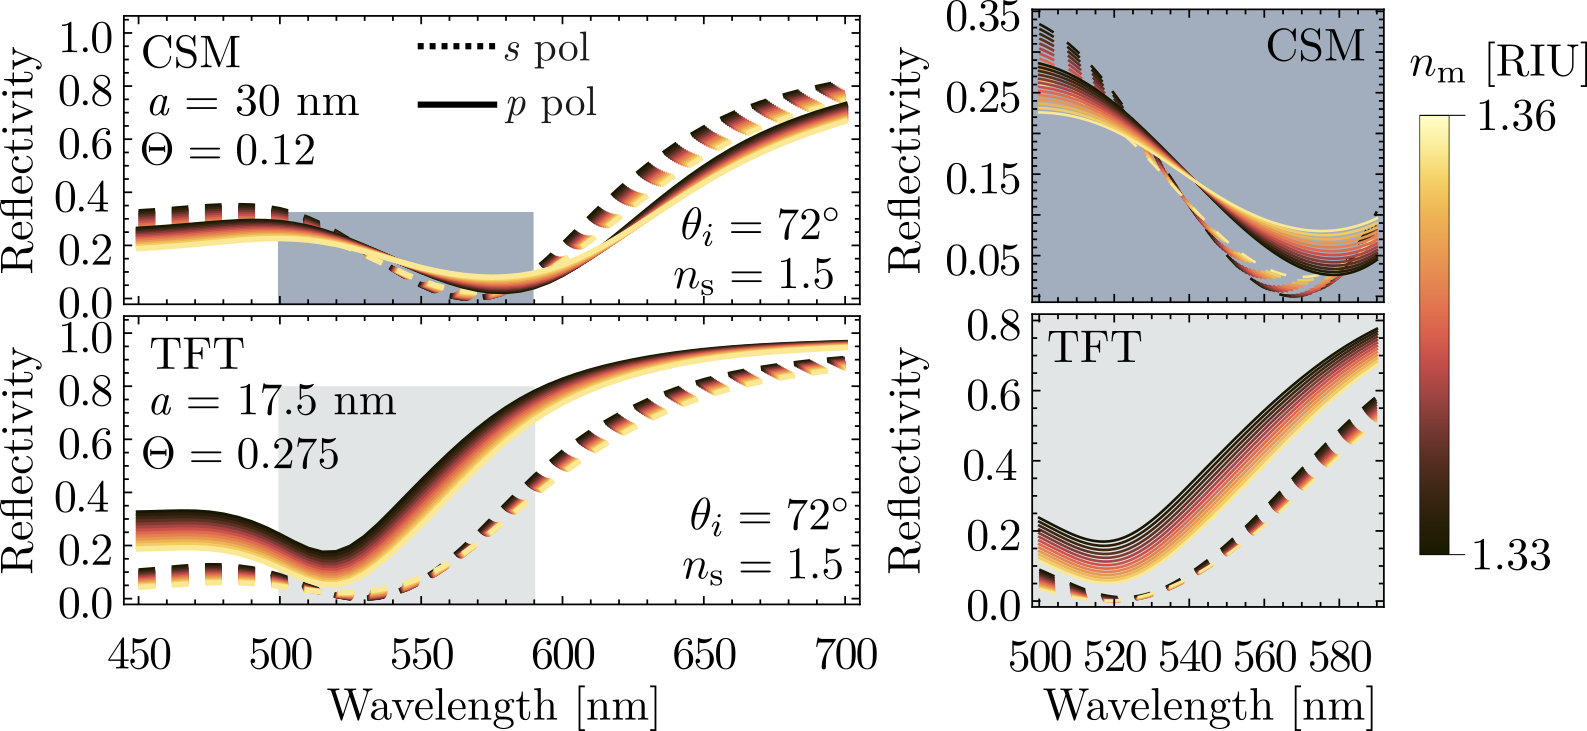
\includegraphics[scale = 1.3]{img/5-Phase/Fig-Refl.png}
\end{frame}



\begin{frame}{\underline{Avances en respuesta óptica y mecanismos de sensado}}
	{Esquema de medición de fase y oscuridad topológica}
	\centering
	\begin{columns}
		\column{\squeezethree}
		\centering	
		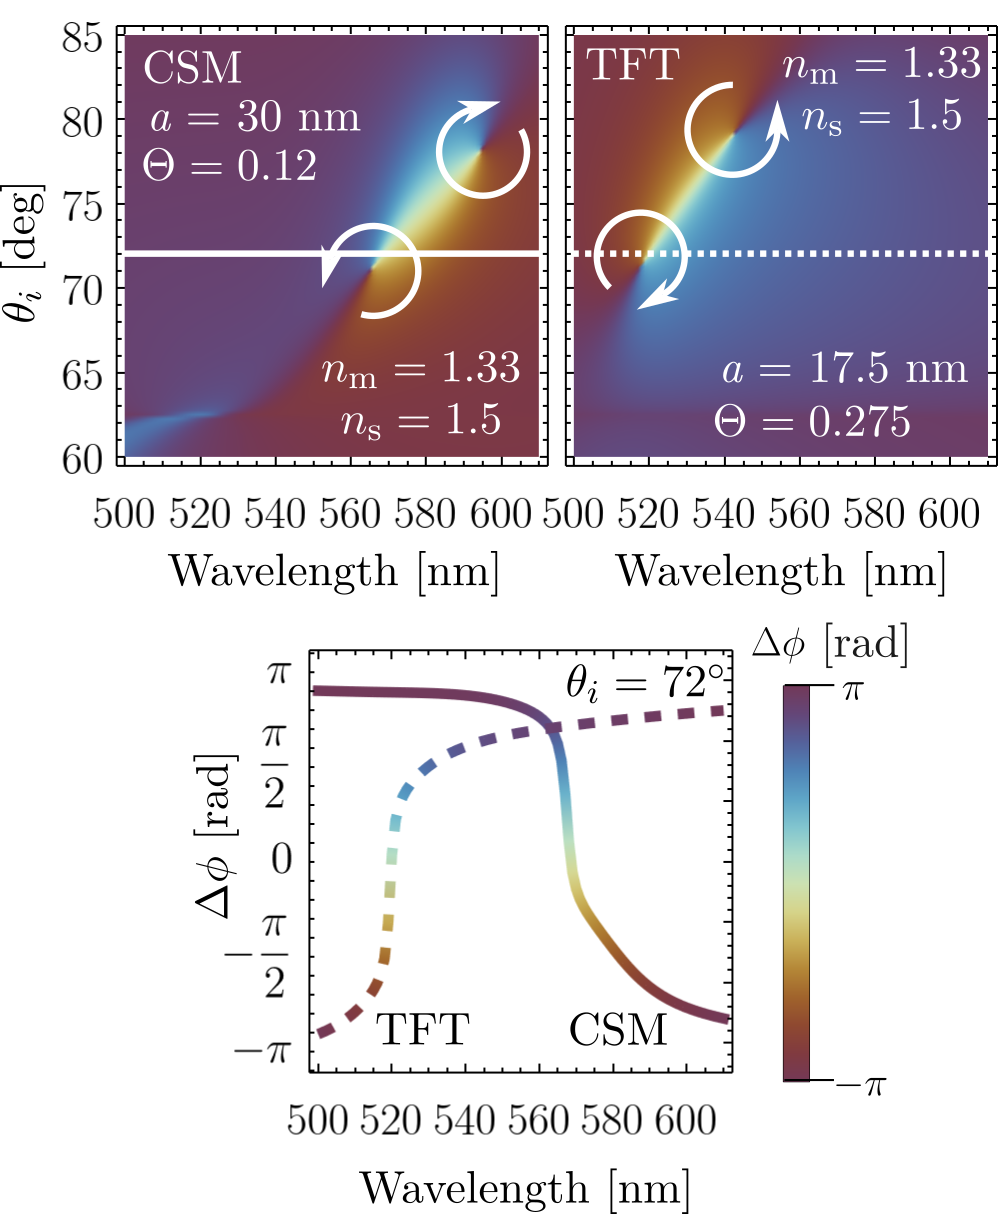
\includegraphics[scale = 1]{img/5-Phase/Fig-TD.png}
		\column{\squeezetwo}
		\centering
		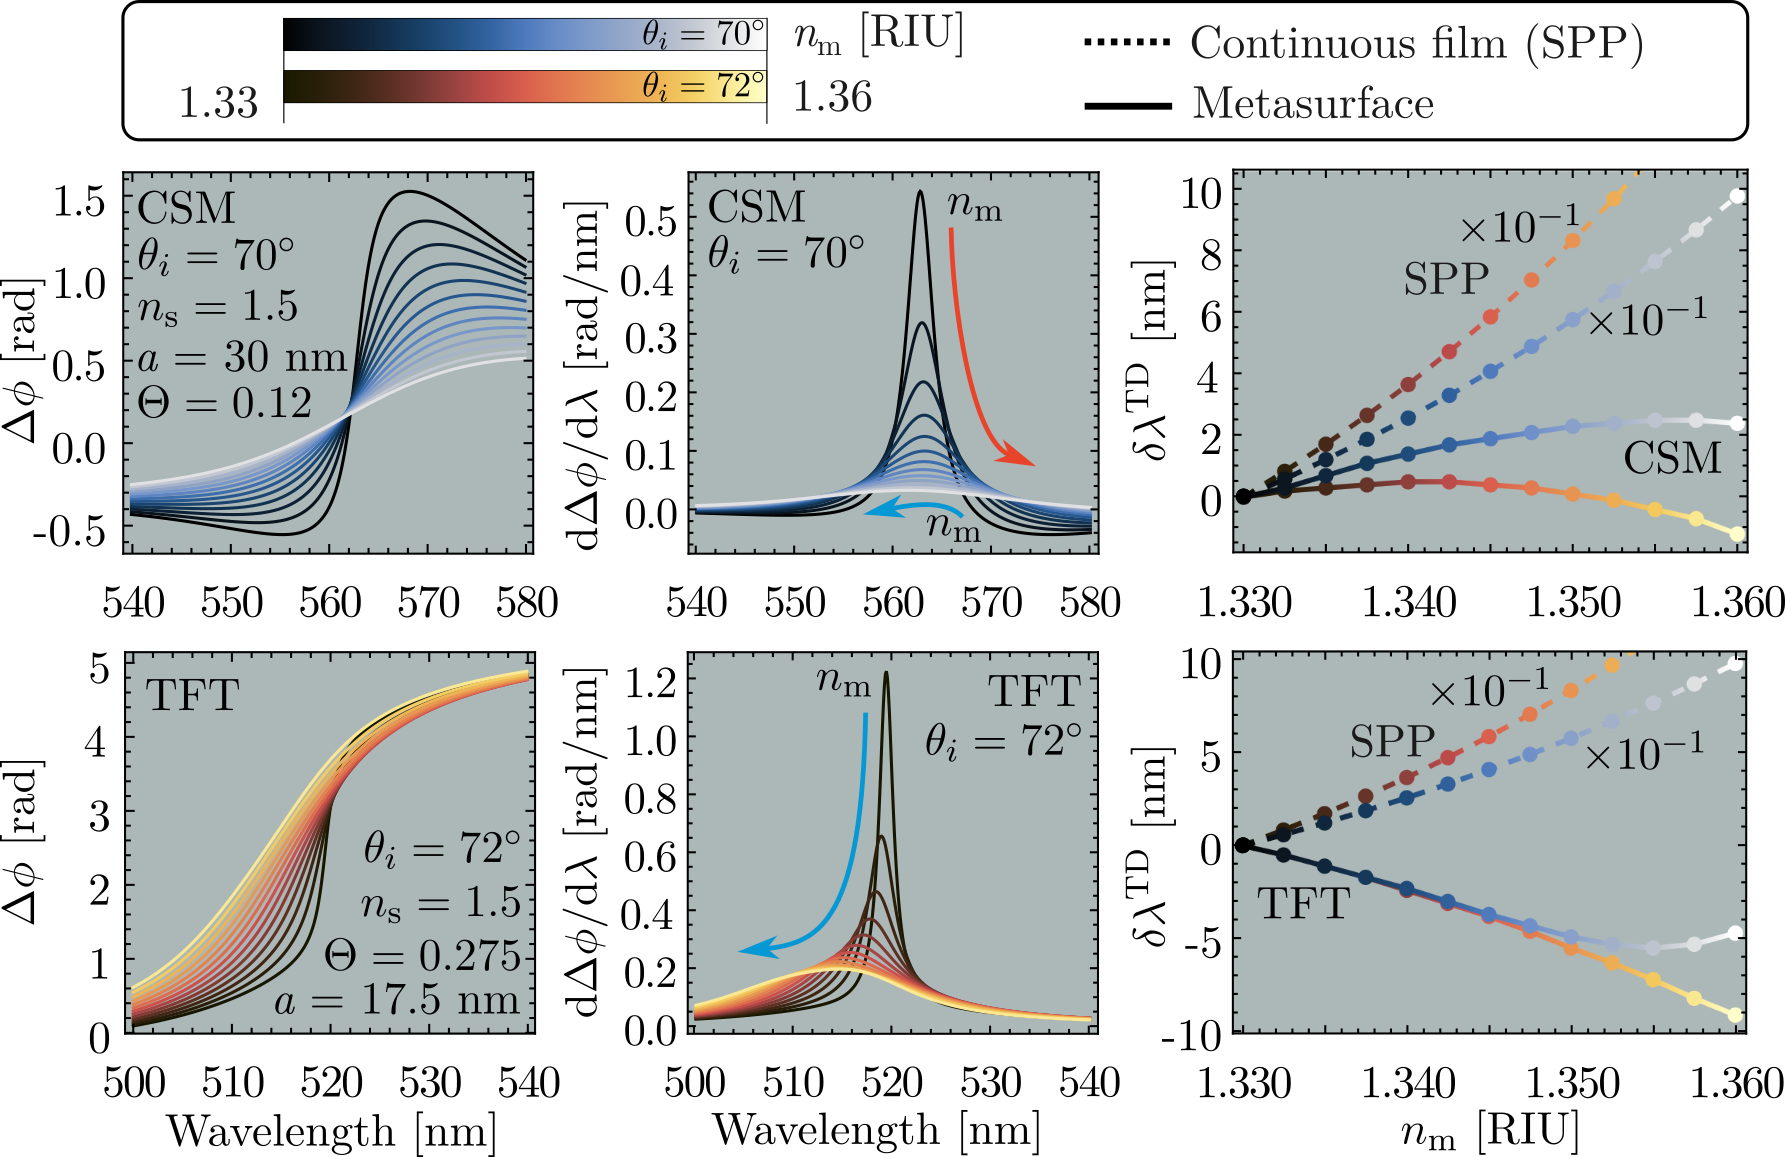
\includegraphics[scale = 1]{img/5-Phase/Fig-Sens.png}
	\end{columns}
\end{frame}

\begin{frame}{\underline{Avances en respuesta óptica y mecanismos de sensado}}
	{Evidencia experimental de corrimiento al azul}
	\centering	
	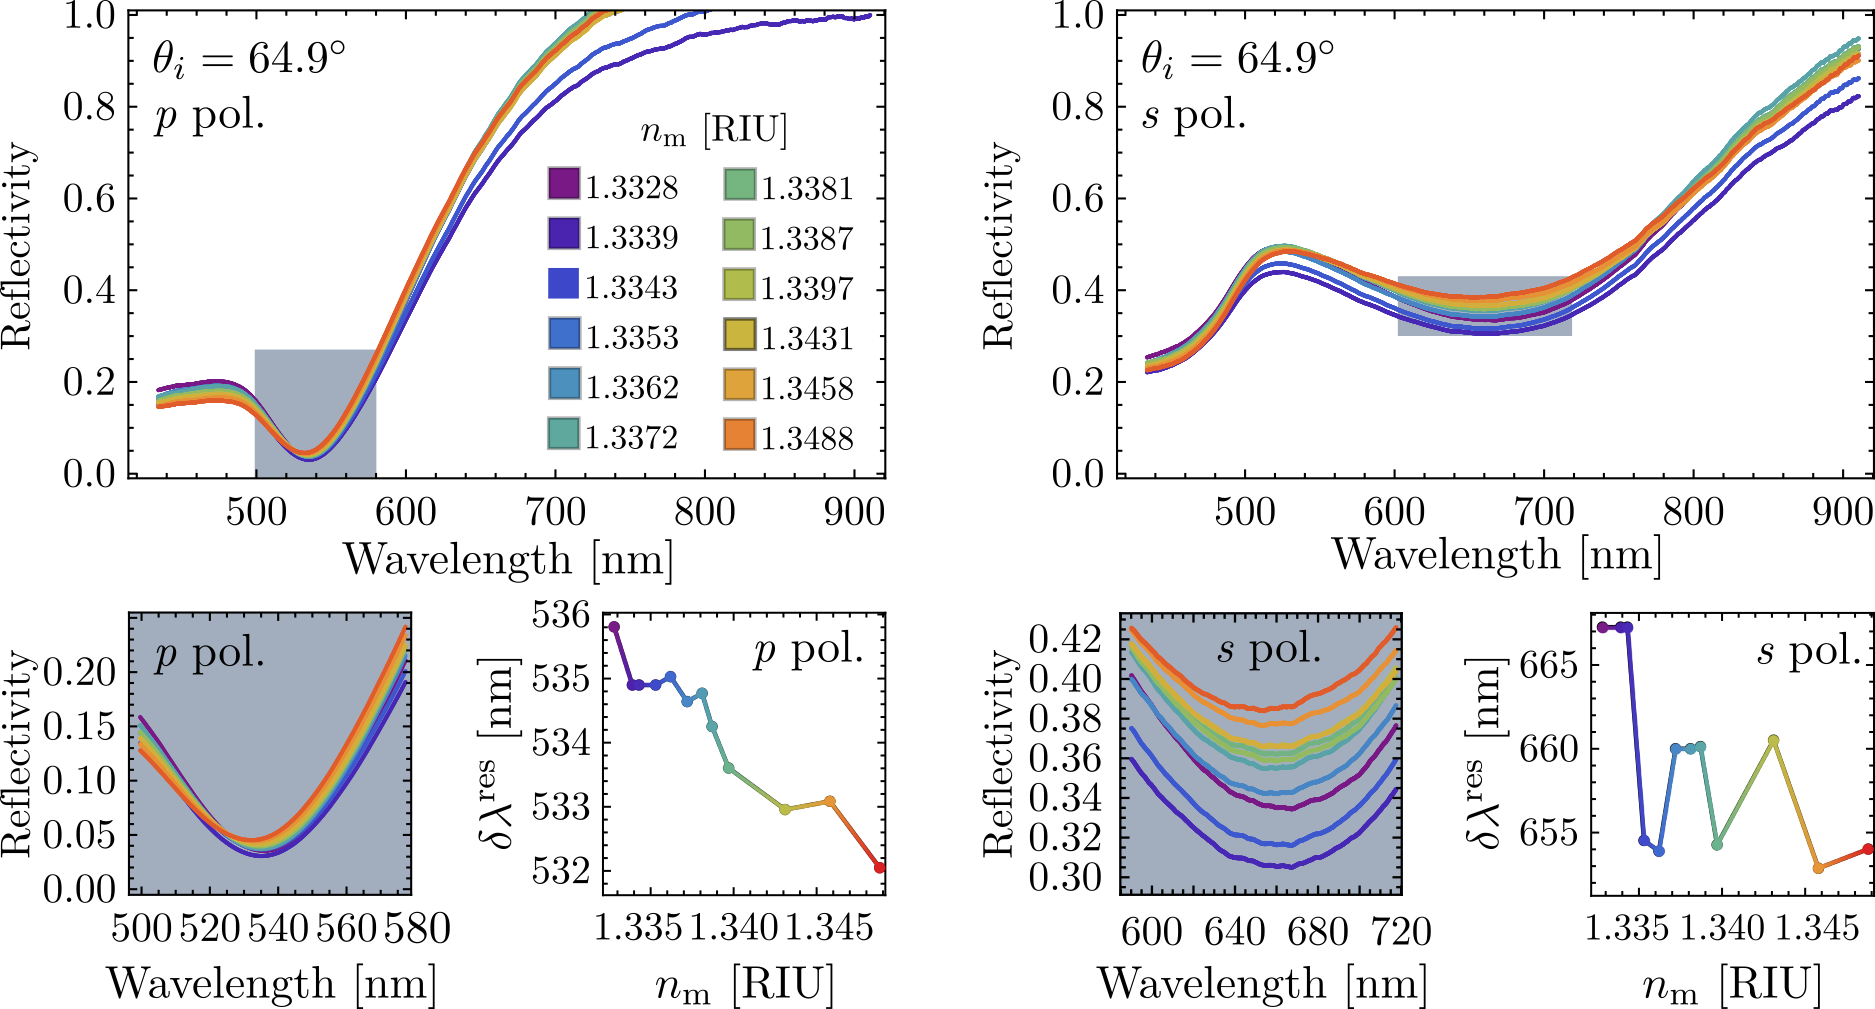
\includegraphics[scale = 1.1]{img/5-Phase/g2.png}
\end{frame}